% =====================================================================
%  Exploring the Mysteries of Flight -- final presentation
%  Tupolev Tu-160 "White Swan"
%
%  Compile with XeLaTeX (twice):
%      latexmk -xelatex main.tex
% =====================================================================
\documentclass[aspectratio=169,t,10pt]{beamer}

\usepackage{bitbeamer}

% ---------------------------------------------------------------------
%  Title block
% ---------------------------------------------------------------------
\title{Tupolev Tu-160}
\subtitle{White Swan: the largest, fastest bomber ever built}
\institute{EXPLORING THE MYSTERIES OF FLIGHT}
\author{Presented by Your Name}
\date{November 2026}

% ---------------------------------------------------------------------
%  Helpers
% ---------------------------------------------------------------------
\newcommand{\outlineentry}[3]{%
  \noindent
  \begin{minipage}[t]{11mm}
    \vspace{0pt}%
    {\color{bitgreen}\fontsize{22}{22}\selectfont\bfseries #1}%
  \end{minipage}%
  \begin{minipage}[t]{52mm}
    \vspace{0.8mm}%
    {\bfseries #2}\par\vspace{0.8mm}%
    {\color{bitgray}\footnotesize #3}%
  \end{minipage}\par\vspace{5.5mm}}

% small grey source line
\newcommand{\src}[1]{\par\vspace{1.6mm}{\color{bitgray}\fontsize{7.2}{8.6}\selectfont #1\par}}

\begin{document}

% ---------------------------------------------------------------- cover
\begin{frame}[plain]
  \titlepage
\end{frame}

% -------------------------------------------------------------- outline
\begin{frame}
  \frametitle{Outline}
  \vspace{2mm}
  \begin{columns}[T]
    \begin{column}{0.48\textwidth}
      \outlineentry{01}{The Aircraft}{Why it exists, and what it is}
      \outlineentry{02}{How It Flies}{Sweep, wave drag and thrust}
    \end{column}
    \begin{column}{0.48\textwidth}
      \outlineentry{03}{Performance}{Standoff strike and service record}
      \outlineentry{04}{Challenges}{Trade-offs, and what remains}
    \end{column}
  \end{columns}
\end{frame}

% ================================================================ PART 1
\bitsectionintro{Role, story and design at a glance}
\section{The Aircraft}

\subsection{Why This Aircraft?}
\begin{frame}
  \frametitle{Why This Aircraft?}
  \begin{columns}[T]
    \begin{column}{0.52\textwidth}
      \begin{itemize}
        \item \bitemph{275 t} at take-off, \bitemph{54.1 m} long, \bitemph{Mach 2.05}
              --- no other bomber combines all three
        \item The last strategic bomber designed in the USSR;
              NATO \bitkw{Blackjack}, Russian \textit{Bely Lebed}, the White Swan
        \item Built around one question: how to put twelve cruise missiles
              on a target 7,000 km away
        \item The answer chosen here was \bitemph{speed, range and payload}
              --- not stealth
      \end{itemize}
    \end{column}
    \begin{column}{0.44\textwidth}
      \centering
      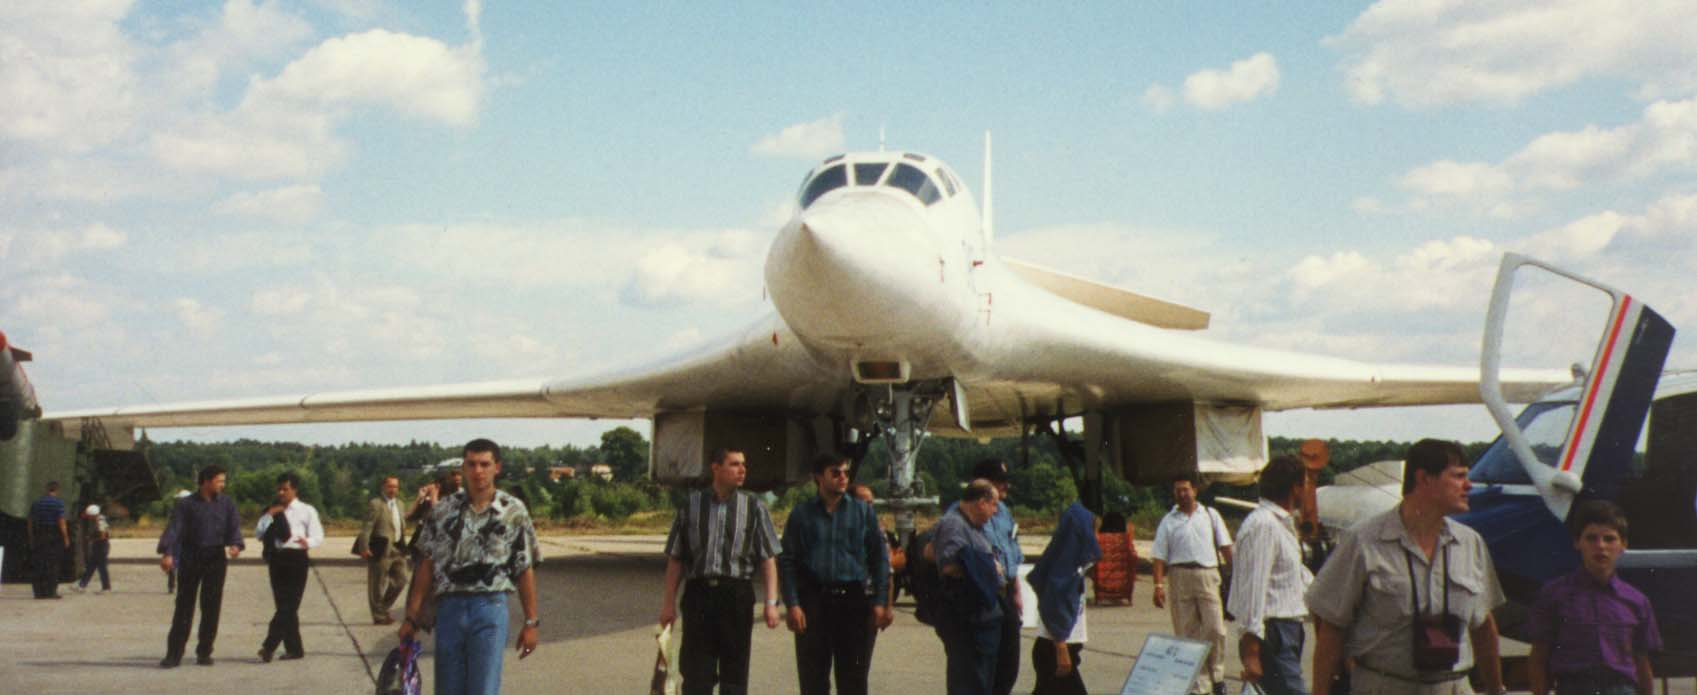
\includegraphics[width=\linewidth]{assets/photos/Tupolev_Tu-160.jpg}
      \vspace{1mm}
      \bitfigcaption{Tu-160 on static display}
      \vspace{0.6mm}
      \src{Photo: Kobel, public domain, via Wikimedia Commons}
    \end{column}
  \end{columns}
\end{frame}

\subsection{Design at a Glance}
\begin{frame}
  \frametitle{Design at a Glance}
  \vspace{-0.5mm}
  {\small
  \renewcommand{\arraystretch}{1.12}%
  \begin{center}
    \begin{bittable}{@{}>{\raggedright\arraybackslash}p{24mm}%
                        >{\raggedright\arraybackslash}p{22mm}%
                        >{\raggedright\arraybackslash}p{20mm}%
                        >{\raggedright\arraybackslash}p{62mm}@{}}
      \toprule
      \textbf{\color{bitgreen}Parameter} &
      \textbf{\color{bitgreen}Tu-160} &
      \textbf{\color{bitgreen}B-1B} &
      \textbf{\color{bitgreen}Why it matters} \\
      \midrule
      Length           & 54.1 m              & 44.5 m        & Volume for fuel and weapon bays \\
      \addlinespace
      Span, 20$^\circ$ / 65$^\circ$ & 55.7 / 35.6 m & 41.8 / 24.1 m & Same sweep logic, larger scale \\
      \addlinespace
      Max take-off     & 275 t               & 216 t         & 27\% more mass to accelerate \\
      \addlinespace
      Max speed        & Mach 2.05           & Mach 1.25     & The design point in one line \\
      \addlinespace
      Internal payload & 45 t                & 34 t          & Twelve missiles instead of eight \\
      \bottomrule
    \end{bittable}
  \end{center}
  }
  \vspace{1.5mm}
  {\small
  Same mission on paper, opposite design point: the B-1B traded Mach 2 for a
  smaller radar signature, the Tu-160 kept the speed. It is 27\% heavier and
  65\% faster --- and visible on radar from much further away.\par}
  \src{Data: Jane's All the World's Aircraft 2003--04 (via Wikipedia); USAF B-1B fact sheet.}
\end{frame}

% ================================================================ PART 2
\bitsectionintro{Sweep, wave drag and thrust}
\section{How It Flies}

\subsection{The Wing, in Numbers}
\begin{frame}
  \frametitle{The Wing, in Numbers}
  \begin{columns}[T]
    \begin{column}{0.53\textwidth}
      \begin{itemize}
        \item A swept wing only feels the flow \textit{normal} to its leading
              edge: $M_n = M\cos\Lambda$
        \item At Mach 2.05: 20$^\circ$ gives $M_n = 1.93$ --- wave drag;
              65$^\circ$ gives 0.87 --- flow stays attached
        \item Sweep costs aspect ratio, 7.8 $\rightarrow$ 3.5, and induced drag
              scales as $1/AR$: 65$^\circ$ only pays when $C_L$ is small
        \item $L/D \approx 18.5$--19 subsonic, above 6 supersonic; stagnation
              125\,$^\circ$C at Mach 2.05 --- hence titanium and a 6\,t hinge
      \end{itemize}
    \end{column}
    \begin{column}{0.43\textwidth}
      \centering
      \begin{tikzpicture}[x=0.66mm,y=15mm]
        \foreach \y in {0.5,1.0,1.5,2.0} {
          \draw[bitline,line width=0.2pt] (0,\y) -- (70,\y);
        }
        \draw[->,bitgray,line width=0.3pt] (0,0) -- (73,0)
          node[right,font=\fontsize{7}{8}\selectfont,text=black] {$\Lambda$ [deg]};
        \draw[->,bitgray,line width=0.3pt] (0,0) -- (0,2.4)
          node[above,font=\fontsize{7}{8}\selectfont,text=black] {$M_n$};
        \foreach \x in {0,20,40,60} {
          \draw[bitgray,line width=0.3pt] (\x,0) -- (\x,-0.04);
          \node[below,font=\fontsize{6.5}{7}\selectfont,text=bitgray] at (\x,0) {\x};
        }
        \foreach \y in {0.5,1.0,1.5,2.0} {
          \node[left,font=\fontsize{6.5}{7}\selectfont,text=bitgray] at (0,\y) {\y};
        }
        \draw[bitred,dashed,line width=0.5pt] (0,1) -- (70,1);
        \node[font=\fontsize{6.5}{7}\selectfont,text=bitred,anchor=west]
          at (2.5,1.12) {$M_n = 1$};
        \draw[bitgreen,line width=1.0pt]
          plot[domain=0:70,samples=100] (\x,{2.05*cos(\x)});
        \fill[bitgreen] (20,{2.05*cos(20)}) circle (0.55mm);
        \node[font=\fontsize{6.5}{7}\selectfont,anchor=south west,text=black]
          at (21,{2.05*cos(20)}) {20$^\circ$: 1.93};
        \fill[bitgreen] (65,{2.05*cos(65)}) circle (0.55mm);
        \node[font=\fontsize{6.5}{7}\selectfont,anchor=north east,text=black]
          at (64,{2.05*cos(65)-0.02}) {65$^\circ$: 0.87};
      \end{tikzpicture}

      \vspace{1mm}
      {\fontsize{7.2}{8.6}\selectfont\color{bitdark}
       Normal Mach number against wing sweep at $M = 2.05$.}
    \end{column}
  \end{columns}
  \src{Own calculation from geometry in Jane's; standard sweep theory, ISA at 12\,km.}
\end{frame}

\subsection{Four NK-32s}
\begin{frame}
  \frametitle{Four NK-32s}
  \begin{columns}[T]
    \begin{column}{0.52\textwidth}
      \begin{itemize}
        \item 4 $\times$ Kuznetsov \bitemph{NK-32} afterburning turbofans:
              137\,kN dry, \bitemph{245\,kN} with reheat
        \item About 980\,kN installed; thrust/weight \bitemph{0.37}
        \item Variable ramps schedule oblique shocks --- pressure recovery is
              what keeps Mach 2 reachable
        \item At $L/D = 6$, drag at 275\,t is $\approx 0.45$\,MN: roughly
              \bitkw{0.5\,MN of excess thrust} for acceleration and climb
      \end{itemize}
    \end{column}
    \begin{column}{0.44\textwidth}
      \centering
      \begin{tikzpicture}[x=1mm,y=1mm]
        % 1 MN = 18 mm
        \def\wA{48.6} % 2.70 MN
        \def\wT{17.6} % 0.98 MN
        \def\wD{8.1}  % 0.45 MN
        \fill[bitgray!40] (0,0) rectangle (\wA,6.5);
        \node[anchor=west,font=\fontsize{6.8}{7.6}\selectfont] at (0.8,3.25)
          {weight 2.70 MN};
        \fill[bitgreen] (0,-13) rectangle (\wT,-13+6.5);
        \node[anchor=west,font=\fontsize{6.8}{7.6}\selectfont,text=bitgreen!60!black]
          at (\wT+0.8,-13+3.25) {thrust 0.98};
        \fill[bitred!80] (0,-26) rectangle (\wD,-26+6.5);
        \node[anchor=west,font=\fontsize{6.8}{7.6}\selectfont,text=bitred!80!black]
          at (\wD+0.8,-26+3.25) {drag 0.45};
        \draw[<->,bitgreen!70!black,line width=0.4pt] (\wD,-31) -- (\wT,-31);
        \node[anchor=north,font=\fontsize{6.4}{7}\selectfont,text=bitgreen!70!black]
          at ({(\wD+\wT)/2},-32) {excess $\approx$ 0.53 MN};
      \end{tikzpicture}

      \vspace{2mm}
      {\fontsize{7.2}{8.6}\selectfont\color{bitdark}
       Forces in MN at 275\,t, Mach 2, $L/D = 6$.}
    \end{column}
  \end{columns}
  \src{Thrust: Jane's (static, reheat). Drag from $D = W/(L/D)$; ram compression raises thrust at Mach 2.}
\end{frame}

% ================================================================ PART 3
\bitsectionintro{Standoff strike and service record}
\section{Performance}

\subsection{Standoff, Not Penetration}
\begin{frame}
  \frametitle{Standoff, Not Penetration}
  \begin{columns}[T]
    \begin{column}{0.56\textwidth}
      \begin{itemize}
        \item Two internal bays, 45\,t, rotary launchers ---
              \bitemph{twelve cruise missiles}
        \item Kh-55SM / Kh-101 / Kh-555, range up to \bitemph{3,000\,km}
        \item Combat radius 7,300\,km subsonic, 2,000\,km at Mach 1.5: the
              aircraft never needs to enter the threat envelope
        \item \bitkw{No defensive armament} --- the first post-war Soviet
              bomber without guns
        \item Survivability comes from distance, not from speed or signature
      \end{itemize}
    \end{column}
    \begin{column}{0.40\textwidth}
      \centering
      \begin{tikzpicture}[x=1mm,y=1mm]
        \foreach \r/\lab in {18/1,0/2} {%
          \draw[bitline,line width=0.4pt,fill=bitlight] (0,\r) rectangle (52,\r+14);
          \node[anchor=south west,font=\fontsize{6}{7}\selectfont,text=bitgray]
            at (0.8,\r+14.2) {bay \lab};
          \foreach \c in {0,...,5} {%
            \begin{scope}[shift={({2.6+8.2*\c},\r+2.8)}]
              \fill[bitgreen!25] (0,0) rectangle (2.2,6.4);
              \draw[bitgreen!70,line width=0.25pt] (0,0) rectangle (2.2,6.4);
              \fill[bitgreen] (1.1,8.7) -- (2.1,6.4) -- (0.1,6.4) -- cycle;
              \fill[bitgreen] (-0.9,0) -- (0.1,1.6) -- (0.1,0) -- cycle;
              \fill[bitgreen] (3.1,0) -- (2.1,1.6) -- (2.1,0) -- cycle;
            \end{scope}
          }
        }
        \node[anchor=north,font=\fontsize{7.2}{8}\selectfont]
          at (26,-4.4) {2 bays $\times$ 6 = 12 missiles};
      \end{tikzpicture}

      \vspace{2mm}
      {\fontsize{7.2}{8.6}\selectfont\color{bitdark}
       Internal carriage only: no external stores, no drag penalty.}
    \end{column}
  \end{columns}
  \src{Armament: Wikipedia (Jane's data); FAS.}
\end{frame}

\subsection{Service Record}
\begin{frame}
  \frametitle{Service Record}
  \vspace{1mm}
  \begin{center}
  \resizebox{0.93\linewidth}{!}{%
  \begin{tikzpicture}[x=1mm,y=1mm]
    \draw[bitline,line width=1.4pt] (0,0) -- (128,0);
    \foreach \i/\yr/\ev/\cl in {%
        0/1981/first flight/bitgreen,
       21/1987/service entry/bitgreen,
       42/1992/production stops/bitgreen,
       63/1999/Ukraine returns 8/bitgreen,
       84/2015/Syria debut/bitgreen,
      105/2022/new-build M/bitred,
      128/2024/in series/bitred} {%
      \fill[\cl] (\i,0) circle (0.95mm);
      \node[above,font=\fontsize{8}{9}\selectfont\bfseries,text=\cl]
        at (\i,1.6) {\yr};
      \node[below,font=\fontsize{6.4}{7.2}\selectfont,text=bitdark,
            align=center,text width=19mm] at (\i,-1.6) {\ev};
    }
  \end{tikzpicture}}
  \end{center}
  \vfill
  \begin{itemize}
    \item $\approx$36 built; about 17 in service with Russian Long-Range Aviation
    \item 44 world records, including a 23-hour, 18,000\,km patrol in 2010
    \item Tu-160M: NK-32-02 engines, new avionics, restarted Kazan line
  \end{itemize}
  \vfill
  \src{Build and fleet numbers: Wikipedia; Airforce Technology.}
\end{frame}

\subsection{The President in the Cockpit}
\begin{frame}
  \frametitle{The President in the Cockpit}
  \begin{columns}[T]
    \begin{column}{0.29\textwidth}
      \centering
      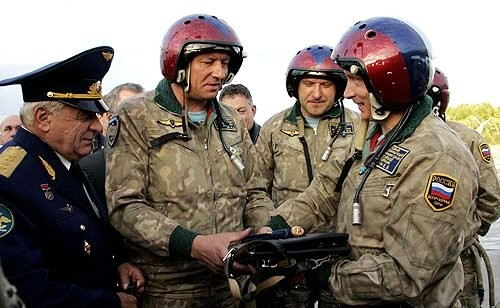
\includegraphics[width=\linewidth]{assets/photos/krem1.jpg}
      \vspace{1mm}
      \bitfigcaption{After the flight, 16 Aug 2005}
      \vspace{0.6mm}
      \src{Photo: kremlin.ru, CC BY 4.0}
    \end{column}
    \begin{column}{0.67\textwidth}
      \small
      {\color{bitgreen}\bfseries 16 August 2005 \textperiodcentered\ Olenegorsk, Kola Peninsula}
      \begin{itemize}
        \item Putin in the \bitemph{commander's seat}, about 5 hours and 5,000\,km
        \item Refuelling, supersonic run, four Kh-555 fired
        \item All four hit a building at the Pemboy range --- two through the
              windows, two through the doors
      \end{itemize}
      \vspace{1mm}
      {\color{bitgreen}\bfseries 22 February 2024 \textperiodcentered\ Kazan}
      \begin{itemize}
        \item 30 minutes in a new-build \bitemph{Tu-160M}, \textit{Ilya Muromets}
        \item ``The technology is excellent. It really belongs to a new generation.''
      \end{itemize}
      \vspace{1.5mm}
      {\itshape Two flights, nineteen years apart: precision in 2005,
       endorsement of the restarted line in 2024.}
    \end{column}
  \end{columns}
  \src{Sources: kremlin.ru (2005, 2024); TASS.}
\end{frame}

% ================================================================ PART 4
\bitsectionintro{Trade-offs and open questions}
\section{Challenges}

\subsection{Trade-offs}
\begin{frame}
  \frametitle{Trade-offs}
  \vspace{-0.5mm}
  {\small
  \renewcommand{\arraystretch}{1.02}%
  \begin{center}
    \begin{bittable}{@{}>{\raggedright\arraybackslash}p{58mm}%
                        >{\raggedright\arraybackslash}p{62mm}@{}}
      \toprule
      \textbf{\color{bitgreen}What the design buys} &
      \textbf{\color{bitred}What it costs} \\
      \midrule
      Range and payload no other bomber matches & Radar cross-section you cannot hide \\
      \addlinespace
      Supersonic dash, short-field capability   & 6\,t hinge, heavy maintenance burden \\
      \addlinespace
      Common systems with Tu-144 and Tu-22M     & Production line cold for 20 years \\
      \addlinespace
      A proven standoff missile platform        & $\approx$17 airframes, high cost per hour \\
      \bottomrule
    \end{bittable}
  \end{center}
  }
  \vspace{2mm}
  \begin{itemize}
    \item Not a stealth aircraft, and never meant to be --- relevance now
          rests on the weapons, not on the airframe
    \item Open question: a missile truck this size, in an age of drones and hypersonics
  \end{itemize}
  \vspace{1.2mm}
  \src{Wikipedia; Airforce Technology.}
\end{frame}

\subsection{Lessons from the Study}
\begin{frame}
  \frametitle{Three Takeaways}
  \vspace{3mm}
  \begin{columns}[T]
    \begin{column}{0.31\textwidth}
      {\color{bitgreen}\fontsize{26}{28}\selectfont\bfseries 01}\par
      \vspace{1mm}
      {\bfseries A clear design point beats a balanced one}\par
      \vspace{1.5mm}
      {\color{bitdark}\small Speed, range and payload --- signature accepted.}
    \end{column}
    \begin{column}{0.31\textwidth}
      {\color{bitgreen}\fontsize{26}{28}\selectfont\bfseries 02}\par
      \vspace{1mm}
      {\bfseries Variable sweep is the enabler and the cost}\par
      \vspace{1.5mm}
      {\color{bitdark}\small Six tonnes of hinge buys Mach 2 and a 3\,km runway.}
    \end{column}
    \begin{column}{0.31\textwidth}
      {\color{bitgreen}\fontsize{26}{28}\selectfont\bfseries 03}\par
      \vspace{1mm}
      {\bfseries Weapons age better than airframes}\par
      \vspace{1.5mm}
      {\color{bitdark}\small New missiles keep a 1981 airframe relevant.}
    \end{column}
  \end{columns}
  \vfill
  \src{All figures: Jane's via Wikipedia; Kremlin; TASS.}
\end{frame}

% --------------------------------------------------------------- closing
\begin{frame}[plain]
  \bitclosingpage{Thank You}{Questions \& discussion}
\end{frame}

\end{document}
